% !TEX root = ../main.tex
\section{METHOD}

\begin{figure*}[t]
  \centering
  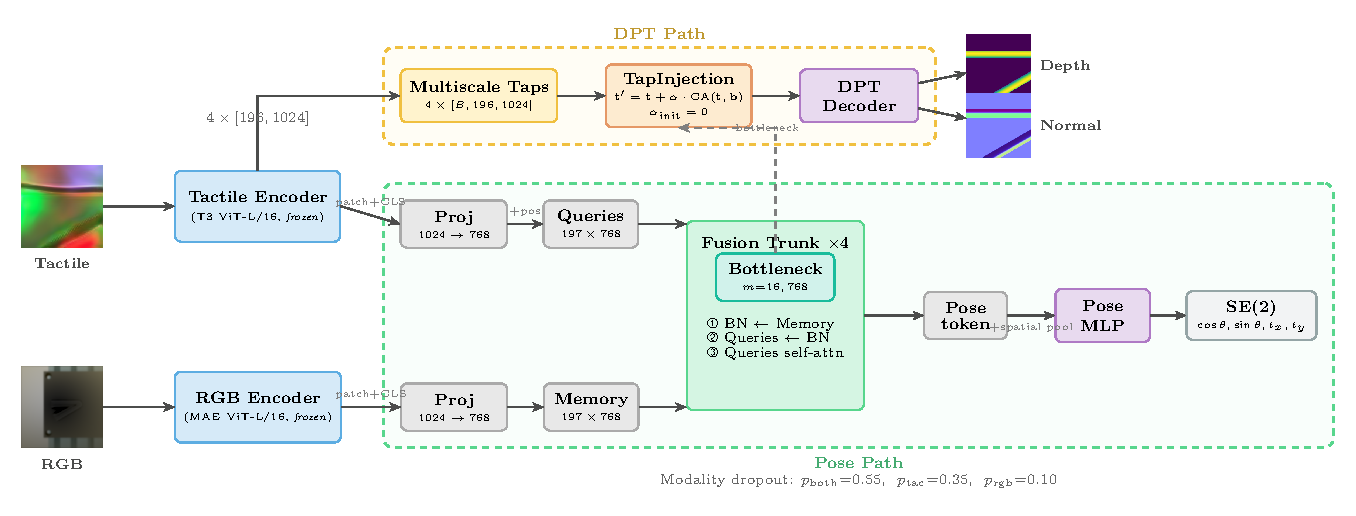
\includegraphics[width=\textwidth]{figures/architecture.pdf}
  \caption{\method{} architecture.
  %
  Frozen modality-specific encoders (T3 for tactile, MAE for RGB) extract
  features at 1024 dimensions. The \textbf{DPT path} (top): multiscale
  encoder taps feed directly into the DPT decoder for depth and normal
  prediction; optional RGB injection via ReZero-gated cross-attention
  ($\alpha$ init${}=0$) from the trunk's bottleneck adds visual context.
  %
  The \textbf{Pose path} (bottom): tactile tokens are projected to 768-dim
  and initialize 197 queries (196 spatial + 1 pose); RGB tokens form the
  read-only memory. A 4-layer asymmetric fusion trunk fuses them through 16
  learnable bottleneck tokens. The resulting pose token feeds an MLP that
  predicts SE(2) pose.
  %
  The decoder receives identical inputs regardless of which modalities are
  present, enabling a single model to serve three inference modes via
  modality dropout.}
  \label{fig:architecture}
\end{figure*}

\subsection{Transparency-Switchable Visuo-Tactile Sensor}
\label{sec:sensor}

\begin{figure}[t]
  \centering
  \todo{Fig.: (a) cross-section of the layer stack (photochromic layer,
  Solaris base, backing plate, UV LEDs, camera); (b) photo of the assembled
  prototype; (c) the same scene imaged in transparent and opaque mode.}
  \caption{Transparency-switchable sensor.
  (a)~Layer stack.
  (b)~Assembled prototype on the robot flange.
  (c)~Transparent mode (UV off) and opaque mode (UV on) views of the same
  contact.}
  \label{fig:sensor}
\end{figure}

GelSight-family sensors~\cite{yuan2017gelsight,donlon2018gelslim} coat the
gel with a permanent opaque reflective layer, which enables photometric
depth reconstruction but blocks the camera's view beyond the contact surface.
Prior dual-mode designs either keep the membrane semi-transparent and switch
by illumination contrast~\cite{hogan2021sts,athar2023vistac,prince2026mvptac},
or keep the gel transparent and track UV-excited
markers~\cite{wang2022spectac,yang2026transtac}, sacrificing part of the
reflective surface that dense reconstruction relies on.
We instead make the reflective layer itself switchable.
Building on the GelSlim~4.0~\cite{sipos2024gelslim4} body, we replace the
blue LEDs of its RGB illumination with UV LEDs and its coated gel with a
photochromic membrane that is transparent by default and turns opaque under
UV (Fig.~\ref{fig:sensor}).

The membrane is a two-layer Solaris\textsuperscript{TM} (Smooth-On) stack.
The 5\,mm base layer is mixed 1:1 by weight, vacuum-degassed, and cast in a
mold; it is optically clear once cured and serves as both the compliant
contact body and the transparent window.
The photochromic layer is spin-coated onto its outer face from 3\,g Solaris
mixed with 0.3\,mL of invisible UV-reactive ink (United Nuclear).
Because both layers are the same silicone, the film deforms with the base
rather than delaminating from it.
The photochromic layer is the outermost surface and contacts the object
directly, with no protective overlayer~\cite{prince2026mvptac}.
In opaque mode the reflective surface therefore coincides with the contact
surface, so the observed shading is produced at the exact geometry being
touched; in transparent mode the optical path contains only two
index-matched silicone layers, avoiding extra interface reflections in the
RGB view.
Despite the exposed surface, the membrane survived more than 40{,}000
contacts in durability testing without loss of switching function.

With UV off, the sensor operates in \emph{transparent mode} and the internal
camera images the external scene through the membrane, yielding $I_r$.
With UV on, the layer switches to an opaque reflective state within
\todo{xx}\,ms, and the remaining red and green LEDs illuminate it for
photometric tactile imaging, yielding $I_t$; the transition reverses
\todo{xx}\,s after UV is removed.
Both images come from the same Raspberry~Pi Zero camera module
(\todo{resolution}) through the same membrane, so they are paired by
construction but not pixel-aligned: the RGB view sees the object and its
surroundings beyond the gel, while the tactile view sees only the contact
patch.
\todo{active area diameter; housing; flange adapter; flex PCB role.}

\subsection{Data Collection}
\label{sec:data_collection}

Each object is rigidly mounted on a square platform attached to a
force--torque (FT) sensor.
Using the robot flange as a probe, we detect sequential edge contacts from
the FT signal, fit the four platform boundaries, and recover the platform
center and in-plane orientation, which define the object frame $\{O\}$ with
$0.1$--$0.2\,$mm in-plane accuracy.
\todo{Add ${}^{W}T_O$, ${}^{O}T_S$ equations if space permits.}

A KUKA LBR Med R820 arm then executes the same trajectory twice.
In Pass~1 the gel is removed and the camera captures a clean reference image
$I_{\text{clean}}^{(i)}$ with the robot pose $P_{\text{robot}}^{(i)}$ at each
waypoint.
In Pass~2 the switchable gel is installed and each waypoint yields a
transparent-mode image $I_{\text{trans}}^{(i)}$ (UV off), an opaque
non-contact background $I_{\text{bg}}^{(i)}$ (UV on), and a tactile image
$I_{\text{tac}}^{(i)}$ (UV on, in contact).
Repeating an identical trajectory maximizes spatial correspondence across
modalities.

\subsection{Problem Formulation}
Given a paired but non-pixel-aligned RGB image $I_r$ and vision-based tactile
image $I_t$, \method{} predicts, in the tactile frame: per-pixel depth $D$,
surface normals $\mathbf{N}$, and the object's planar pose
$(\theta, t_x, t_y) \in SE(2)$.

\subsection{Frozen Modality-Specific Encoders}
\label{sec:encoders}

Each modality is encoded by a frozen pretrained ViT-L encoder selected through
systematic ablation (Sec.~\ref{sec:encoder_ablation}): T3~\cite{zhao2024transferable}
for tactile and MAE~\cite{he2022mae} for RGB, both producing 1024-dim features
with 196 patch tokens ($14{\times}14$ grid at patch size 16).

Freezing serves two purposes.
First, it \emph{anchors sim-to-real transfer}: because the encoder weights are
never updated on simulated data, the feature space inherits the pretraining
distribution, bridging the sim-real domain gap without explicit adaptation.
Second, it ensures \emph{ablation fairness}: the trainable parameter count is
identical across all modality configurations, so no encoder capacity can shift
between modes.

Using separate, modality-matched encoders rather than a single shared backbone
yields an additional benefit: each encoder's inductive bias is tailored to its
input domain. T3's sensor-specific front-end captures gel-deformation patterns
that a generic vision encoder may overlook, while MAE's reconstruction-based
pretraining produces features well-suited to appearance-based recognition.

\subsection{Asymmetric Bottleneck Fusion Trunk}
\label{sec:trunk}

The fusion trunk operates at $D{=}768$ dimensions after a learned linear
projection from the encoder's native 1024-dim space. A separate
\texttt{BranchProjection} (linear + learned modality embedding) is applied to
each modality's tokens.

Tactile is the spatial anchor: its 196 projected patch tokens, augmented with
a learned spatial positional embedding, initialize the \emph{spatial queries};
its CLS token initializes the \emph{pose query} (197 queries total). RGB's
projected patch and CLS tokens form the read-only \emph{memory}
($197$ key-value tokens).

Each of the $L{=}4$ fusion layers applies three sequential attention steps:
\begin{enumerate}
\item \textbf{Bottleneck $\leftarrow$ Memory} (cross-attention, no FFN):
      $m{=}16$ learnable bottleneck tokens attend to the 197 RGB memory tokens,
      compressing RGB context into a compact representation.
\item \textbf{Queries $\leftarrow$ Bottleneck} (cross-attention + FFN):
      the 197 queries read from the $m$ bottleneck tokens, gating how much RGB
      information enters the tactile-anchored representation.
\item \textbf{Queries $\leftarrow$ Queries} (self-attention + FFN):
      queries refine amongst themselves.
\end{enumerate}
Because attention output length follows the query count, the trunk output is
always 197 tokens at 768-dim regardless of whether RGB is present. The
bottleneck tokens persist across layers (\emph{carry} mode), accumulating
progressively refined RGB context.

An optional per-object embedding $\mathbf{e}_{\mathrm{obj}} \in
\mathbb{R}^{768}$ is added to all 197 queries to provide object identity for
pose disambiguation across multiple objects.

\subsection{Decoupled Dense and Pose Paths}
\label{sec:decoupled}

The dense prediction and pose estimation paths are architecturally decoupled
to prevent modality dropout from diluting dense supervision.

\paragraph{DPT path.}
The DPT decoder~\cite{ranftl2021dpt} taps the \emph{tactile encoder}
directly at its native 1024-dim multiscale features, extracted at four
intermediate layers (layers 5, 11, 17, 23 of the 24-layer ViT). Each tap
receives a learned positional embedding before entering the DPT reassembly
($\text{Conv}_{1{\times}1}$: $1024 {\to} 256$, bilinear rescale) and
fusion-upsampling pipeline, producing depth ($C{=}1$) and surface normals
($C{=}3$) at the input resolution of $224{\times}224$.

Because the DPT path bypasses the fusion trunk, the pose-path modality
dropout never dilutes its tactile input: whenever the tactile image is
present (the \emph{both} and \emph{tactile} configurations, 90\% of steps)
the decoder sees pure tactile taps. In the RGB-only configuration the same
decoder falls back to the RGB encoder's multiscale taps, which is possible
because both encoders share the ViT-L token geometry (196 tokens, 1024-dim);
this yields a coarse shape prior rather than contact geometry
(Table~\ref{tab:modality_ablation}).

\paragraph{RGB injection via TapInjection.}
When RGB is available, visual context is optionally injected into the DPT taps
through a residual cross-attention mechanism with a ReZero gate:
\begin{equation}
  \mathbf{t}'_i = \mathbf{t}_i + \alpha_i \cdot
    \mathrm{CrossAttn}(\mathbf{t}_i,\, \mathbf{b})
  \label{eq:tap_inject}
\end{equation}
where $\mathbf{t}_i \in \mathbb{R}^{196 \times 1024}$ is the $i$-th encoder
tap, $\mathbf{b} \in \mathbb{R}^{16 \times 768}$ is the trunk bottleneck
(projected to 1024-dim for key/value), and $\alpha_i$ is a learnable scalar
initialized to zero. This ensures the DPT path starts as a pure
tactile-encoder pipeline and gradually learns to incorporate RGB context.
Injection is independently sampled per training step ($p = 0.5$), further
decoupling it from the pose path's modality dropout.

\paragraph{Pose path.}
After the fusion trunk, the pose token $\mathbf{p} \in \mathbb{R}^{768}$ and
mean-pooled spatial queries $\bar{\mathbf{s}} \in \mathbb{R}^{768}$ are
concatenated ($\mathbb{R}^{1536}$) and decoded by a 3-layer MLP to produce
$(\cos\theta, \sin\theta, t_x, t_y)$. The first two outputs are
L2-normalized to enforce unit-circle structure.

\subsection{Three Configurations, One Shared Model}
\label{sec:three_configs}

The model is trained with modality dropout: each step randomly samples one of
three input configurations with probabilities
$p_{\text{both}}{=}0.55$, $p_{\text{tactile}}{=}0.35$,
$p_{\text{rgb}}{=}0.10$.
%
At inference, these become three modes of the same trained weights:
\begin{itemize}
\item \textbf{RGB+tactile}: all three trunk steps run; DPT receives tactile
      taps with optional RGB injection.
\item \textbf{Tactile-only}: steps 1--2 are skipped (no RGB memory); only
      self-attention (step 3) refines the queries. DPT receives pure tactile taps.
\item \textbf{RGB-only}: learned mask tokens replace tactile queries; all
      three trunk steps run. DPT falls back to RGB encoder taps.
\end{itemize}
Importantly, the decoder input shape is identical in all three modes, so the
comparison is not confounded by architectural differences.

\subsection{Loss Functions and Training}
\label{sec:losses}

\paragraph{Task losses.}
Depth is supervised with MSE loss; surface normals with MSE loss; rotation
with $\mathcal{L}_{\text{rot}} = 1 - (\cos\hat\theta \cos\theta^*
+ \sin\hat\theta \sin\theta^*)$ (equivalent to $1 - \cos(\Delta\theta)$);
translation with L1 loss on $(t_x, t_y)$.

\paragraph{Grouped uncertainty weighting.}
Following~\cite{kendall2018multi}, we learn per-task homoscedastic uncertainty
terms, but group them into a \emph{dense} group (depth + normals) and a
\emph{pose} group (rotation + translation):
\begin{equation}
  \mathcal{L} = \lambda \sum_{i \in \text{dense}}
    \bigl(e^{-s_i}\mathcal{L}_i + \tfrac{1}{2}s_i\bigr)
  + \sum_{j \in \text{pose}}
    \bigl(e^{-s_j}\mathcal{L}_j + \tfrac{1}{2}s_j\bigr)
\end{equation}
where $s_i$ are learned log-variances and $\lambda$ is a fixed ratio between
groups. Grouping prevents pose improvements from starving dense gradients.

\paragraph{Training details.}
We train with AdamW ($\text{lr}{=}2 \times 10^{-4}$,
$\text{wd}{=}0.05$), cosine schedule with 1000-step linear warmup, for 150
epochs at batch size 64 per GPU on 2 GPUs (effective batch 128). Mixed
precision (fp16) and gradient clipping ($\|\cdot\| \leq 1.0$) are used
throughout. Only the projections, embeddings, bottleneck, fusion trunk, and
heads are trainable (${\sim}95$M of ${\sim}398$M total parameters).

\paragraph{Augmentation.}
Tactile images undergo heavy photometric augmentation---per-channel gain/bias,
directional gradients, residual noise, and Gaussian noise---to simulate sensor
variability across gel specimens and lighting conditions. RGB images receive
lighter, uniform-channel augmentation to preserve marker hue. Both modalities
undergo a fixed $1/\sqrt{2}$ center crop (eliminating border artifacts under
rotation augmentation) followed by a random gel-spin rotation
$\phi \sim \mathcal{U}(-180^{\circ}, 180^{\circ})$.

\paragraph{Sim+real co-training.}
\todo{Describe the simulated dataset (TACTO / other sim, objects, number of
samples) and the optimal real:sim ratio finding (1:2.7).}
